\section{Unknown Token [UNK]}

The unknown token, denoted as \unk{}, represents one of the oldest and most fundamental special tokens in natural language processing. Despite the evolution of sophisticated subword tokenization methods, the \unk{} token remains crucial for handling out-of-vocabulary (OOV) words and understanding the robustness limits of language models. This section explores its historical significance, modern applications, and the ongoing challenge of vocabulary coverage in transformer models.

\subsection{The Out-of-Vocabulary Problem}

Natural language contains an effectively infinite vocabulary due to:

\begin{itemize}
\item \textbf{Morphological Productivity}: Languages continuously create new word forms through inflection and derivation
\item \textbf{Named Entities}: Proper nouns, technical terms, and domain-specific vocabulary
\item \textbf{Borrowing and Code-Mixing}: Words from other languages and mixed-language texts
\item \textbf{Neologisms}: New words coined for emerging concepts and technologies
\item \textbf{Typos and Variations}: Misspellings, abbreviations, and informal variants
\end{itemize}

Fixed-vocabulary models must handle these unknown words, traditionally through the \unk{} token mechanism.

\subsection{Traditional UNK Token Approach}

\subsubsection{Vocabulary Construction}
In early neural language models, vocabulary construction followed a frequency-based approach:

\begin{enumerate}
\item Collect a large training corpus
\item Count word frequencies
\item Select the top-K most frequent words (typically K = 30,000-50,000)
\item Replace all other words with \unk{} during preprocessing
\end{enumerate}

\subsubsection{Training and Inference}
During training, the model learns to:
\begin{itemize}
\item Predict \unk{} for low-frequency words
\item Use \unk{} representations for downstream tasks
\item Handle \unk{} tokens in various contexts
\end{itemize}

During inference, any word not in the vocabulary is mapped to \unk{}.

\begin{lstlisting}[language=Python, caption=Traditional UNK Processing]
class TraditionalTokenizer:
    def __init__(self, vocab_size=30000):
        self.vocab_size = vocab_size
        self.word_to_id = {}
        self.id_to_word = {}
        self.unk_token = "[UNK]"
        self.unk_id = 0
        
    def build_vocab(self, texts):
        # Count word frequencies
        word_counts = {}
        for text in texts:
            for word in text.split():
                word_counts[word] = word_counts.get(word, 0) + 1
        
        # Sort by frequency and take top K
        sorted_words = sorted(word_counts.items(), 
                            key=lambda x: x[1], reverse=True)
        
        # Build vocabulary
        self.word_to_id[self.unk_token] = self.unk_id
        self.id_to_word[self.unk_id] = self.unk_token
        
        for i, (word, count) in enumerate(sorted_words[:self.vocab_size-1]):
            word_id = i + 1
            self.word_to_id[word] = word_id
            self.id_to_word[word_id] = word
            
    def encode(self, text):
        tokens = []
        for word in text.split():
            if word in self.word_to_id:
                tokens.append(self.word_to_id[word])
            else:
                tokens.append(self.unk_id)  # Map to UNK
        return tokens
    
    def decode(self, token_ids):
        words = []
        for token_id in token_ids:
            if token_id in self.id_to_word:
                words.append(self.id_to_word[token_id])
            else:
                words.append(self.unk_token)
        return " ".join(words)

# Example usage
tokenizer = TraditionalTokenizer(vocab_size=1000)

# Build vocabulary from training data
training_texts = [
    "the quick brown fox jumps over the lazy dog",
    "natural language processing is fascinating",
    "transformers revolutionized machine learning"
]
tokenizer.build_vocab(training_texts)

# Handle OOV words
test_text = "the sophisticated algorithm demonstrates remarkable performance"
encoded = tokenizer.encode(test_text)
decoded = tokenizer.decode(encoded)

print(f"Original: {test_text}")
print(f"Encoded:  {encoded}")
print(f"Decoded:  {decoded}")
# Output might be: "the [UNK] [UNK] [UNK] [UNK] [UNK]"
\end{lstlisting}

\subsection{Limitations of Traditional UNK Approach}

The traditional \unk{} token approach suffers from several critical limitations:

\subsubsection{Information Loss}
When multiple different words are mapped to the same \unk{} token:
\begin{itemize}
\item Semantic information is completely lost
\item Morphological relationships are ignored
\item Context-specific meanings cannot be distinguished
\end{itemize}

\subsubsection{Poor Handling of Morphologically Rich Languages}
Languages with extensive inflection and agglutination suffer particularly:
\begin{itemize}
\item Each inflected form may be treated as a separate word
\item Vocabulary explosion leads to excessive \unk{} usage
\item Morphological compositionality is not captured
\end{itemize}

\subsubsection{Domain Adaptation Challenges}
Models trained on one domain struggle with others:
\begin{itemize}
\item Technical vocabulary becomes predominantly \unk{}
\item Domain-specific terms lose all semantic content
\item Transfer learning effectiveness is severely limited
\end{itemize}

\subsubsection{Generation Quality Degradation}
During text generation:
\begin{itemize}
\item \unk{} tokens produce meaningless outputs
\item Vocabulary limitations constrain expressiveness
\item Post-processing is required to handle \unk{} tokens
\end{itemize}

\subsection{The Subword Revolution}

The limitations of \unk{} tokens drove the development of subword tokenization methods:

\subsubsection{Byte Pair Encoding (BPE)}
BPE iteratively merges the most frequent character pairs:
\begin{itemize}
\item Starts with character-level vocabulary
\item Gradually builds up common subwords
\item Rare words are decomposed into known subwords
\item Eliminates most \unk{} tokens
\end{itemize}

\subsubsection{WordPiece}
Used in BERT and similar models:
\begin{itemize}
\item Similar to BPE but optimizes likelihood on training data
\item Uses \texttt{\#\#} prefix to mark subword continuations
\item Balances vocabulary size with semantic coherence
\end{itemize}

\subsubsection{SentencePiece}
A unified subword tokenizer:
\begin{itemize}
\item Treats text as raw byte sequences
\item Handles multiple languages uniformly
\item Includes whitespace in the subword vocabulary
\end{itemize}

\begin{lstlisting}[language=Python, caption=Subword vs Traditional Tokenization]
from transformers import BertTokenizer, GPT2Tokenizer

# Traditional word-level tokenizer (conceptual)
def traditional_tokenize(text, vocab):
    tokens = []
    for word in text.split():
        if word.lower() in vocab:
            tokens.append(word.lower())
        else:
            tokens.append("[UNK]")
    return tokens

# Modern subword tokenizers
bert_tokenizer = BertTokenizer.from_pretrained('bert-base-uncased')
gpt2_tokenizer = GPT2Tokenizer.from_pretrained('gpt2')

# Test with a sentence containing rare words
text = "The antidisestablishmentarianism movement was extraordinarily complex"

# Traditional approach (simulated)
simple_vocab = {"the", "was", "movement", "complex"}
traditional_result = traditional_tokenize(text, simple_vocab)
print(f"Traditional: {traditional_result}")
# Output: ['the', '[UNK]', 'movement', 'was', '[UNK]', 'complex']

# BERT WordPiece
bert_tokens = bert_tokenizer.tokenize(text)
print(f"BERT WordPiece: {bert_tokens}")
# Output: ['the', 'anti', '##dis', '##esta', '##bli', '##sh', '##ment', '##arian', '##ism', 'movement', 'was', 'extraordinary', 'complex']

# GPT-2 BPE
gpt2_tokens = gpt2_tokenizer.tokenize(text)
print(f"GPT-2 BPE: {gpt2_tokens}")
# Output shows subword breakdown without UNK tokens

# Check for UNK tokens
bert_has_unk = '[UNK]' in bert_tokens
gpt2_has_unk = '<|endoftext|>' in gpt2_tokens  # GPT-2's special token
print(f"BERT has UNK: {bert_has_unk}")
print(f"GPT-2 has UNK: {gpt2_has_unk}")
\end{lstlisting}

\subsection{UNK Tokens in Modern Transformers}

Despite subword tokenization, \unk{} tokens haven't disappeared entirely:

\subsubsection{Character-Level Fallbacks}
Some tokenizers still use \unk{} for:
\begin{itemize}
\item Characters outside the supported Unicode range
\item Extremely rare character combinations
\item Corrupted or malformed text
\end{itemize}

\subsubsection{Domain-Specific Vocabularies}
Specialized models may still encounter \unk{} tokens:
\begin{itemize}
\item Mathematical symbols and equations
\item Programming language syntax
\item Domain-specific notation systems
\end{itemize}

\subsubsection{Multilingual Challenges}
Even advanced subword methods struggle with:
\begin{itemize}
\item Scripts not represented in training data
\item Code-switching between languages
\item Historical or archaic language variants
\end{itemize}

\begin{figure}[h]
\centering
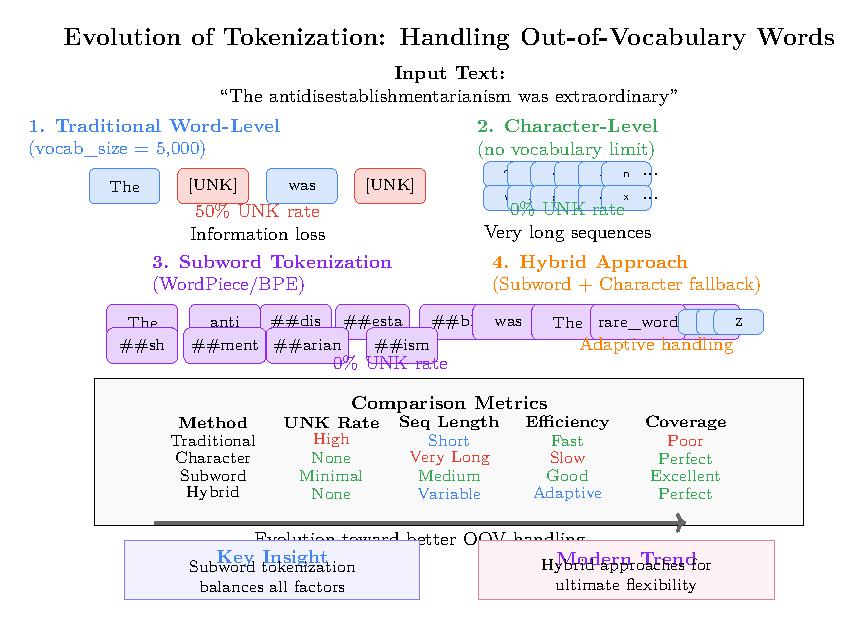
\includegraphics[width=0.9\textwidth]{part1/chapter02/fig_tokenization_comparison.pdf}
\caption{Comparison of tokenization strategies and their handling of out-of-vocabulary words}
\end{figure}

\subsection{Handling UNK Tokens in Practice}

\subsubsection{Training Strategies}
When \unk{} tokens are present:

\begin{itemize}
\item \textbf{UNK Smoothing}: Randomly replace low-frequency words with \unk{} during training
\item \textbf{UNK Replacement}: Use placeholder tokens that can be post-processed
\item \textbf{Copy Mechanisms}: Allow models to copy from input when generating \unk{}
\end{itemize}

\subsubsection{Inference Handling}
Strategies for dealing with \unk{} tokens during inference:

\begin{lstlisting}[language=Python, caption=UNK Token Handling]
import torch
from transformers import BertTokenizer, BertForMaskedLM

def handle_unk_prediction(text, model, tokenizer):
    """Handle prediction when UNK tokens are present."""
    
    # Tokenize input
    inputs = tokenizer(text, return_tensors='pt')
    tokens = tokenizer.convert_ids_to_tokens(inputs['input_ids'][0])
    
    # Find UNK positions
    unk_positions = [i for i, token in enumerate(tokens) 
                    if token == tokenizer.unk_token]
    
    if not unk_positions:
        return text, []  # No UNK tokens
    
    predictions = []
    
    for pos in unk_positions:
        # Mask the UNK token
        masked_inputs = inputs['input_ids'].clone()
        masked_inputs[0, pos] = tokenizer.mask_token_id
        
        # Predict the masked token
        with torch.no_grad():
            outputs = model(masked_inputs)
            logits = outputs.logits[0, pos]
            predicted_id = torch.argmax(logits).item()
            predicted_token = tokenizer.decode([predicted_id])
            
        predictions.append((pos, predicted_token))
    
    return text, predictions

# Example usage
tokenizer = BertTokenizer.from_pretrained('bert-base-uncased')
model = BertForMaskedLM.from_pretrained('bert-base-uncased')

# Text with potential UNK tokens
text = "The researcher studied quantum computing applications"
result, unk_predictions = handle_unk_prediction(text, model, tokenizer)

print(f"Original: {text}")
if unk_predictions:
    print("UNK token predictions:")
    for pos, prediction in unk_predictions:
        print(f"  Position {pos}: {prediction}")
else:
    print("No UNK tokens found")
\end{lstlisting}

\subsection{UNK Token Analysis and Debugging}

\subsubsection{Vocabulary Coverage Analysis}
Understanding \unk{} token frequency helps assess model limitations:

\begin{lstlisting}[language=Python]
def analyze_vocabulary_coverage(texts, tokenizer):
    """Analyze UNK token frequency across texts."""
    
    total_tokens = 0
    unk_count = 0
    unk_words = set()
    
    for text in texts:
        tokens = tokenizer.tokenize(text)
        words = text.split()
        
        total_tokens += len(tokens)
        
        for word in words:
            word_tokens = tokenizer.tokenize(word)
            if tokenizer.unk_token in word_tokens:
                unk_count += len([t for t in word_tokens 
                                if t == tokenizer.unk_token])
                unk_words.add(word)
    
    coverage = (total_tokens - unk_count) / total_tokens if total_tokens > 0 else 0
    
    return {
        'total_tokens': total_tokens,
        'unk_count': unk_count,
        'coverage_rate': coverage,
        'unk_words': list(unk_words)
    }

# Example analysis
texts = [
    "Standard English text with common words",
    "Technical jargon: photosynthesis, mitochondria, ribosomes",
    "Foreign words: schadenfreude, saudade, ubuntu"
]

analysis = analyze_vocabulary_coverage(texts, tokenizer)
print(f"Vocabulary coverage: {analysis['coverage_rate']:.2%}")
print(f"UNK words found: {analysis['unk_words']}")
\end{lstlisting}

\subsubsection{Domain Adaptation Assessment}
Measuring \unk{} token frequency helps evaluate domain transfer:

\begin{itemize}
\item High \unk{} frequency indicates poor domain coverage
\item Specific \unk{} patterns reveal vocabulary gaps
\item Domain-specific vocabulary analysis guides model selection
\end{itemize}

\subsection{Alternatives and Modern Solutions}

\subsubsection{Character-Level Models}
Some approaches eliminate \unk{} tokens entirely:
\begin{itemize}
\item Process text at character level
\item Can handle any Unicode character
\item Computationally expensive for long sequences
\end{itemize}

\subsubsection{Hybrid Approaches}
Combine multiple strategies:
\begin{itemize}
\item Primary subword tokenization
\item Character-level fallback for \unk{} tokens
\item Context-aware token replacement
\end{itemize}

\subsubsection{Dynamic Vocabularies}
Emerging techniques for adaptive vocabularies:
\begin{itemize}
\item Online vocabulary expansion
\item Context-dependent tokenization
\item Learned token boundaries
\end{itemize}

\subsection{UNK Tokens in Evaluation and Metrics}

\subsubsection{Impact on Evaluation}
\unk{} tokens affect various metrics:
\begin{itemize}
\item \textbf{BLEU Score}: \unk{} tokens typically count as mismatches
\item \textbf{Perplexity}: \unk{} token probability affects language model evaluation
\item \textbf{Downstream Tasks}: \unk{} tokens can degrade task performance
\end{itemize}

\subsubsection{Evaluation Best Practices}
\begin{itemize}
\item Report \unk{} token rates alongside primary metrics
\item Analyze \unk{} token impact on different text types
\item Consider domain-specific vocabulary coverage
\end{itemize}

\subsection{Future Directions}

\subsubsection{Contextualized UNK Handling}
Future developments may include:
\begin{itemize}
\item Context-aware \unk{} token representations
\item Learned strategies for \unk{} token processing
\item Dynamic vocabulary expansion during inference
\end{itemize}

\subsubsection{Cross-Lingual UNK Mitigation}
Multilingual models may develop:
\begin{itemize}
\item Cross-lingual transfer for \unk{} tokens
\item Universal character-level representations
\item Language-adaptive tokenization strategies
\end{itemize}

\begin{principle}[UNK Token Best Practices]
\begin{enumerate}
\item \textbf{Minimize Occurrence}: Use appropriate subword tokenization to reduce \unk{} frequency
\item \textbf{Monitor Coverage}: Regularly analyze vocabulary coverage for target domains
\item \textbf{Handle Gracefully}: Implement robust strategies for \unk{} token processing
\item \textbf{Evaluate Impact}: Assess how \unk{} tokens affect downstream task performance
\item \textbf{Document Limitations}: Clearly communicate vocabulary limitations to users
\end{enumerate}
\end{principle}

\subsection{Conclusion}

The \unk{} token represents both a practical necessity and a fundamental limitation in language modeling. While modern subword tokenization methods have dramatically reduced \unk{} token frequency, they haven't eliminated the underlying challenge of open vocabulary processing. Understanding \unk{} token behavior, implementing appropriate handling strategies, and recognizing their impact on model performance remains crucial for effective transformer deployment.

As language models continue to evolve toward more dynamic and adaptive architectures, the role of \unk{} tokens will likely transform from a necessary evil to a bridge toward more sophisticated vocabulary handling mechanisms. The lessons learned from decades of \unk{} token management inform current research into universal tokenization, cross-lingual representation, and adaptive vocabulary systems that promise to further expand the capabilities of transformer-based language understanding.